% questions.tex —— 2010 年·普通高等学校招生考试·江西卷·理科 · 题目内容片段（无答案）
% 由 tools/generate_projects.py 依来源总账自 2010/2010_数学真题_江西理_试题.md 生成，勿手改（改源 MD 后重跑）


状态：needs-review；依固定候选 PDF 两页（印刷页 607–608）逐题核验，五幅图已矢量重绘。原页未印分值，不补。

\gkpart{一、选择题}

\begin{question}
\gkti{1}已知 $(x+\mathrm i)(1-\mathrm i)=y$，则实数 $x,y$ 分别为（　）

（A）$x=-1$，$y=1$

（B）$x=-1$，$y=2$

（C）$x=1$，$y=1$

（D）$x=1$，$y=2$

\end{question}
\begin{question}
\gkti{2}已知集合 $A=\{x\mid |x|\leqslant1,\ x\in\mathbf R\}$，$B=\{y\mid y=x^2,\ x\in\mathbf R\}$，则 $A\cap B=$（　）

（A）$\{x\mid -1\leqslant x\leqslant1\}$

（B）$\{x\mid x\geqslant0\}$

（C）$\{x\mid 0\leqslant x\leqslant1\}$

（D）$\varnothing$

\end{question}
\begin{question}
\gkti{3}不等式 $\dfrac{|x-2|}{x}>\dfrac{x-2}{x}$ 的解集是（　）

（A）$(0,2)$

（B）$(-\infty,0)$

（C）$(2,+\infty)$

（D）$(-\infty,0)\cup(0,+\infty)$

\end{question}
\begin{question}
\gkti{4}$\lim\limits_{n\to\infty}\left(1+\dfrac13+\dfrac1{3^2}+\cdots+\dfrac1{3^n}\right)=$（　）

（A）$\frac53$

（B）$\frac32$

（C）$2$

（D）不存在

\end{question}
\begin{question}
\gkti{5}等比数列 $\{a_n\}$ 中，$a_1=2$，$a_8=4$，函数 $f(x)=x(x-a_1)(x-a_2)\cdots(x-a_8)$，则 $f'(0)=$（　）

（A）$2^6$

（B）$2^9$

（C）$2^{12}$

（D）$2^{15}$

\end{question}
\begin{question}
\gkti{6}$(2-\sqrt x)^8$ 展开式中不含 $x^4$ 项的系数的和为（　）

（A）$-1$

（B）$0$

（C）$1$

（D）$2$

\end{question}
\begin{question}
\gkti{7}$E$，$F$ 是等腰直角 $\triangle ABC$ 斜边 $AB$ 上的三等分点，则 $\tan\angle ECF=$（　）

（A）$\frac{16}{27}$

（B）$\frac23$

（C）$\frac{\sqrt3}3$

（D）$\frac34$

\end{question}
\begin{question}
\gkti{8}直线 $y=kx+3$ 与圆 $(x-3)^2+(y-2)^2=4$ 相交于 $M$，$N$ 两点，若 $|MN|\geqslant2\sqrt3$，则 $k$ 的取值范围是（　）

（A）$\left[-\frac34,0\right]$

（B）$\left(-\infty,-\frac34\right]\cup[0,+\infty)$

（C）$\left[-\frac{\sqrt3}3,\frac{\sqrt3}3\right]$

（D）$\left[-\frac23,0\right]$

\end{question}
\begin{question}
\gkti{9}给出下列三个命题：

① 函数 $y=\dfrac12\ln\dfrac{1-\cos x}{1+\cos x}$ 与 $y=\ln\tan\dfrac x2$ 是同一函数；

② 若函数 $y=f(x)$ 与 $y=g(x)$ 的图象关于直线 $y=x$ 对称，则函数 $y=f(2x)$ 与 $y=\dfrac12g(x)$ 的图象也关于直线 $y=x$ 对称；

③ 若奇函数 $f(x)$ 对定义域内任意 $x$ 都有 $f(x)=f(2-x)$，则 $f(x)$ 为周期函数。

其中真命题是（　）

（A）①②

（B）①③

（C）②③

（D）②

\Needspace{0.4\textheight}
\end{question}
\begingroup
\renewenvironment{question}{\Needspace{0.5\textheight}}{}
\begin{question}
\gkti{10}过正方体 $ABCD-A_1B_1C_1D_1$ 的顶点 $A$ 作直线 $l$，使 $l$ 与棱 $AB$，$AD$，$AA_1$ 所成的角都相等，这样的直线 $l$ 可以作（　）

（A）$1$ 条

（B）$2$ 条

（C）$3$ 条

（D）$4$ 条
\nopagebreak[4]
\begin{center}% 2010 年江西卷理科第 10 题：正方体 ABCD-A1B1C1D1（过顶点 A 作与 AB、AD、AA1 成等角的直线）。
% 来源 PDF：普通高考/2010/2010江西理.pdf，SHA-256 994a56c33da151e22af3fabe292d1b5b193866dfc35773a4431e6dfc8a0cc934。
% 原页：第 1 页（A3 三栏）第 2 栏上部，书页码 607。
% 重绘依据：照原页视角，前面为 B-C-C1-B1，后面为 A-D-D1-A1（后脸右上偏移）；
%   不可见棱 A-A1、A1-D1、A1-B1 画虚线。
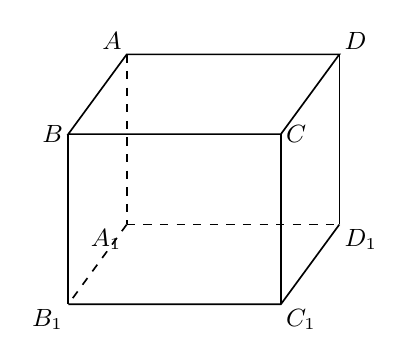
\begin{tikzpicture}[semithick, scale=1.35, every node/.style={inner sep=1.6pt, font=\small}]
  \coordinate (B) at (0,0);
  \coordinate (C) at (2,0);
  \coordinate (C1) at (2,-1.6);
  \coordinate (B1) at (0,-1.6);
  \coordinate (A) at (0.55,0.75);
  \coordinate (D) at (2.55,0.75);
  \coordinate (D1) at (2.55,-0.85);
  \coordinate (A1) at (0.55,-0.85);
  % 可见面与棱
  \draw (A) -- (B) -- (C) -- (D) -- cycle;
  \draw (B) -- (B1);
  \draw (C) -- (C1);
  \draw (D) -- (D1);
  \draw (B1) -- (C1) -- (D1);
  % 不可见棱
  \draw[dashed] (A) -- (A1);
  \draw[dashed] (A1) -- (D1);
  \draw[dashed] (A1) -- (B1);
  \node[above left] at (A) {$A$};
  \node[above right] at (D) {$D$};
  \node[left] at (B) {$B$};
  \node[right] at (C) {$C$};
  \node[below left] at (A1) {$A_1$};
  \node[below right] at (D1) {$D_1$};
  \node[below left] at (B1) {$B_1$};
  \node[below right] at (C1) {$C_1$};
\end{tikzpicture}
\end{center}
\nopagebreak[4]
\end{question}
\endgroup
\begin{question}
\gkti{11}一位国王的铸币大臣在每箱 $100$ 枚的硬币中各掺入了一枚劣币，国王怀疑大臣作弊，他用两种方法来检测。方法一：在 $10$ 箱中各任意抽查一枚；方法二：在 $5$ 箱中各任意抽查两枚。国王用方法一、二能发现至少一枚劣币的概率分别记为 $p_1$ 和 $p_2$。则（　）

（A）$p_1=p_2$

（B）$p_1<p_2$

（C）$p_1>p_2$

（D）以上三种情况都有可能

\Needspace{0.4\textheight}
\end{question}
\begingroup
\renewenvironment{question}{\Needspace{0.5\textheight}}{}
\begin{question}
\gkti{12}如图，一个正五角星薄片（其对称轴与水面垂直）匀速地升出水面，记 $t$ 时刻五角星露出水面部分的图形面积为 $S(t)$（$S(0)=0$），则导函数 $y=S'(t)$ 的图象大致为（　）
\nopagebreak[4]
\begin{center}% 2010 年江西卷理科第 12 题：水中的正五角星与四个导函数图象选项。
% 来源 PDF：普通高考/2010/2010江西理.pdf，SHA-256 994a56c33da151e22af3fabe292d1b5b193866dfc35773a4431e6dfc8a0cc934。
% 原页：第 1 页（A3 三栏）第 2 栏中部，书页码 607。
% 重绘依据：照原页，正五角星（角尖向上）浸在圆柱水柱内，星顶在筒口以下；
%   水面为筒内的虚线椭圆，星的两条下臂尖没入水面以下；正确答案 D：S' 正比于
%   水面截线长度，由 0 增到下方凹角处的局部极大、略降、再升到最宽处、最后降到 0，且连续。
% 说明：四幅导函数图为按题设定性特征绘制的示意（原页每幅宽不足 3cm）。
\begin{tikzpicture}[semithick]
  % ---- 上半：圆柱与五角星 ----
  \begin{scope}[shift={(0,0)}]
    % 圆柱：上沿实线椭圆，两侧母线，下沿虚线椭圆
    \draw (0,0) ellipse (1.9 and 0.5);
    \draw (-1.9,0) -- (-1.9,-2.5);
    \draw (1.9,0) -- (1.9,-2.5);
    \draw[dashed] (0,-2.5) ellipse (1.9 and 0.5);
    % 正五角星：外接圆半径 1.12，圆心 (0,-1.2)
    \begin{scope}[shift={(0,-1.2)},scale=1.12]
      \fill[gray!55] (90:1) -- (162:0.382) -- (234:1) -- (306:0.382) -- (18:1)
        -- (54:0.382) -- (126:1) -- (198:0.382) -- (270:1) -- (342:0.382) -- cycle;
      \draw (90:1) -- (162:0.382) -- (234:1) -- (306:0.382) -- (18:1)
        -- (54:0.382) -- (126:1) -- (198:0.382) -- (270:1) -- (342:0.382) -- cycle;
    \end{scope}
    % 水面：筒内虚线椭圆（压在星上，表示没入水中的部分）
    \draw[dashed] (0,-1.55) ellipse (1.9 and 0.5);
  \end{scope}
  % ---- 下半：四个选项 ----
  % (A) 有断点与尖峰
  \begin{scope}[shift={(-0.2,-5.0)}]
    \draw[-stealth] (-0.35,0) -- (2.0,0) node[right] {$t$};
    \draw[-stealth] (0,-0.55) -- (0,1.05) node[above] {$y$};
    \node[below left] at (0,0) {$O$};
    \draw (0,0) -- (0.55,0.28);
    \draw[fill=white] (0.55,0.28) circle (1.4pt);
    \draw[fill=white] (0.62,0.72) circle (1.4pt);
    \draw (0.62,0.72) -- (1.05,0.42) -- (1.28,0.55) -- (1.55,0.1);
    \draw (1.28,0.55) -- (1.44,0.78) -- (1.62,0.1);
    \node at (0.85,-0.95) {（A）};
  \end{scope}
  % (B) 先升后骤降并穿越横轴
  \begin{scope}[shift={(2.9,-5.0)}]
    \draw[-stealth] (-0.35,0) -- (2.0,0) node[right] {$t$};
    \draw[-stealth] (0,-0.85) -- (0,0.8) node[above] {$y$};
    \node[below left] at (0,0) {$O$};
    \draw (0.0,-0.02) -- (0.5,0.22) -- (0.66,0.3);
    \draw (0.66,0.66) -- (0.9,0.34) -- (1.2,-0.62);
    \draw (0.66,0.3) -- (0.66,0.66);
    \draw (1.2,-0.62) -- (1.42,0.1) -- (1.62,-0.12) -- (1.9,0.2);
    \node at (0.85,-1.2) {（B）};
  \end{scope}
  % (C) 单调递增
  \begin{scope}[shift={(6.0,-5.0)}]
    \draw[-stealth] (-0.35,0) -- (2.0,0) node[right] {$t$};
    \draw[-stealth] (0,-0.5) -- (0,1.15) node[above] {$y$};
    \node[below left] at (0,0) {$O$};
    \draw (0,0) -- (0.5,0.3) -- (0.75,0.45) -- (0.78,0.78) -- (1.05,0.9) -- (1.35,1.02);
    \node at (0.85,-0.95) {（C）};
  \end{scope}
  % (D) 升—略降—再升到最高—降到 0
  \begin{scope}[shift={(9.1,-5.0)}]
    \draw[-stealth] (-0.35,0) -- (2.1,0) node[right] {$t$};
    \draw[-stealth] (0,-0.5) -- (0,1.15) node[above] {$y$};
    \node[below left] at (0,0) {$O$};
    \draw (0,0) -- (0.45,0.42) -- (0.62,0.4) -- (1.05,0.95) -- (1.25,0.68) -- (1.55,0.62) -- (1.82,0);
    \node at (0.9,-0.95) {（D）};
  \end{scope}
\end{tikzpicture}
\end{center}
\nopagebreak[4]
\end{question}
\endgroup
\gkpart{二、填空题}

\begin{question}
\gkti{13}已知向量 $\boldsymbol a$，$\boldsymbol b$ 满足 $|\boldsymbol a|=1$，$|\boldsymbol b|=2$，$\boldsymbol a$ 与 $\boldsymbol b$ 的夹角为 $60^\circ$，则 $|\boldsymbol a-\boldsymbol b|=$ $\underline{\qquad}$。

\end{question}
\begin{question}
\gkti{14}将 $6$ 位志愿者分成 $4$ 组，其中两个组各 $2$ 人，另两个组各 $1$ 人，分赴世博会的四个不同场馆服务，不同的分配方案有$\underline{\qquad}$种。（用数字作答）

\end{question}
\begin{question}
\gkti{15}点 $A(x_0,y_0)$ 在双曲线 $\dfrac{x^2}{4}-\dfrac{y^2}{32}=1$ 的右支上，若点 $A$ 到右焦点的距离等于 $2x_0$，则 $x_0=$ $\underline{\qquad}$。

\Needspace{0.4\textheight}
\end{question}
\begingroup
\renewenvironment{question}{\Needspace{0.5\textheight}}{}
\begin{question}
\gkti{16}如图，在三棱锥 $O-ABC$ 中，三条棱 $OA$，$OB$，$OC$ 两两垂直，且 $OA>OB>OC$，分别经过三条棱 $OA$，$OB$，$OC$ 作一个截面平分三棱锥的体积，截面面积依次为 $S_1$，$S_2$，$S_3$，则 $S_1$，$S_2$，$S_3$ 的大小关系为$\underline{\qquad}$。
\nopagebreak[4]
\begin{center}% 2010 年江西卷理科第 16 题：三棱锥 O-ABC（OA、OB、OC 两两垂直）。
% 来源 PDF：普通高考/2010/2010江西理.pdf，SHA-256 994a56c33da151e22af3fabe292d1b5b193866dfc35773a4431e6dfc8a0cc934。
% 原页：第 1 页（A3 三栏）第 2 栏下部，书页码 607。
% 重绘依据：照原页，O 在上，A 左下，B 右下，C 在右侧中部；OA、OB、OC 为三条两两垂直的棱，
%   可见棱 OA、OB、OC、AB、BC 画实线，被面 OAB 遮挡的棱 AC 画虚线。
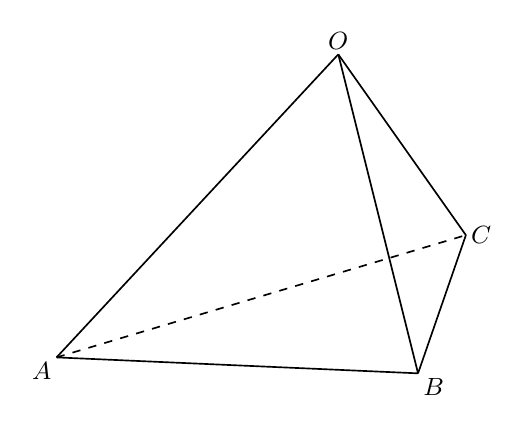
\begin{tikzpicture}[semithick, scale=1.35, every node/.style={inner sep=1.6pt, font=\small}]
  \coordinate (O) at (0.35,1.85);
  \coordinate (A) at (-2.3,-1.0);
  \coordinate (B) at (1.1,-1.15);
  \coordinate (C) at (1.55,0.15);
  \draw (O) -- (A);
  \draw (O) -- (B);
  \draw (O) -- (C);
  \draw (A) -- (B);
  \draw (B) -- (C);
  \draw[dashed] (A) -- (C);
  \node[above] at (O) {$O$};
  \node[below left] at (A) {$A$};
  \node[below right] at (B) {$B$};
  \node[right] at (C) {$C$};
\end{tikzpicture}
\end{center}
\nopagebreak[4]
\end{question}
\endgroup
\gkpart{三、解答题}

\begin{question}
\gkti{17}已知函数 $f(x)=(1+\cot x)\sin^2x+m\sin\left(x+\dfrac\pi4\right)\sin\left(x-\dfrac\pi4\right)$。

（1）当 $m=0$ 时，求 $f(x)$ 在区间 $\left[\dfrac\pi8,\dfrac{3\pi}4\right]$ 上的取值范围；

（2）当 $\tan\alpha=2$ 时，$f(\alpha)=\dfrac35$，求 $m$ 的值。

\end{question}
\begin{question}
\gkti{18}某迷宫有三个通道，进入迷宫的每个人都要经过一个智能门。首次到达此门，系统会随机（即等可能）为你打开一个通道。若是 $1$ 号通道，则需要 $1$ 小时走出迷宫；若是 $2$ 号、$3$ 号通道，则分别需要 $2$ 小时、$3$ 小时返回智能门。再次到达智能门时，系统会随机打开一个你未到过的通道，直至走出迷宫为止。令 $\xi$ 表示走出迷宫所需的时间。

（1）求 $\xi$ 的分布列；

（2）求 $\xi$ 的数学期望。

\end{question}
\begin{question}
\gkti{19}设函数 $f(x)=\ln x+\ln(2-x)+ax$（$a>0$）。

（1）当 $a=1$ 时，求 $f(x)$ 的单调区间；

（2）若 $f(x)$ 在 $(0,1]$ 上的最大值为 $\dfrac12$，求 $a$ 的值。

\Needspace{0.4\textheight}
\end{question}
\begingroup
\renewenvironment{question}{\Needspace{0.5\textheight}}{}
\begin{question}
\gkti{20}如图，$\triangle BCD$ 与 $\triangle MCD$ 都是边长为 $2$ 的正三角形，平面 $MCD\perp$ 平面 $BCD$，$AB\perp$ 平面 $BCD$，$AB=2\sqrt3$。

（1）求点 $A$ 到平面 $MBC$ 的距离；

（2）求平面 $ACM$ 与平面 $BCD$ 所成二面角的正弦值。
\nopagebreak[4]
\begin{center}% 2010 年江西卷理科第 20 题：两个共边正三角形 BCD、MCD 与垂线段 AB。
% 来源 PDF：普通高考/2010/2010江西理.pdf，SHA-256 994a56c33da151e22af3fabe292d1b5b193866dfc35773a4431e6dfc8a0cc934。
% 原页：第 2 页（A3 三栏）第 1 栏中部，书页码 608。
% 重绘依据：照原页视角，A 在 B 正上方（AB⊥底面），C 在下，D 在右，M 在 CD 中点的正上方
%   （平面 MCD⊥平面 BCD）；可见棱 AB、AC、AD、AM、BC、CD、MC、MD 画实线，BD、BM 画虚线。
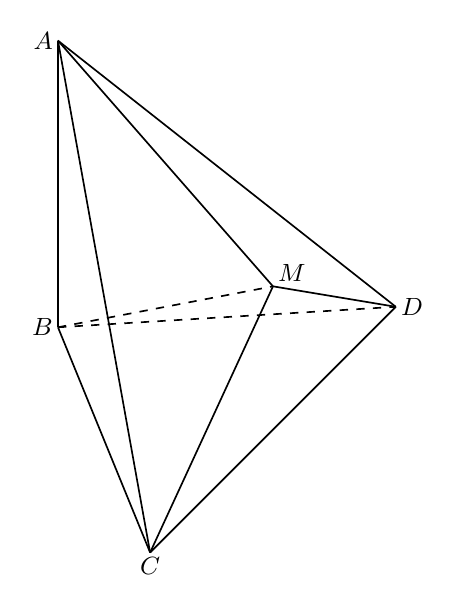
\begin{tikzpicture}[semithick, scale=1.3, every node/.style={inner sep=1.6pt, font=\small}]
  \coordinate (B) at (0,0);
  \coordinate (A) at (0,2.8);
  \coordinate (C) at (0.9,-2.2);
  \coordinate (D) at (3.3,0.2);
  \coordinate (M) at (2.1,0.4);
  \draw (A) -- (B);
  \draw (A) -- (C);
  \draw (A) -- (D);
  \draw (A) -- (M);
  \draw (B) -- (C);
  \draw (C) -- (D);
  \draw (M) -- (C);
  \draw (M) -- (D);
  \draw[dashed] (B) -- (D);
  \draw[dashed] (B) -- (M);
  \node[left] at (A) {$A$};
  \node[left] at (B) {$B$};
  \node[below] at (C) {$C$};
  \node[right] at (D) {$D$};
  \node[above right] at (M) {$M$};
\end{tikzpicture}
\end{center}
\nopagebreak[4]
\Needspace{0.4\textheight}
\end{question}
\endgroup
\begingroup
\renewenvironment{question}{\Needspace{0.5\textheight}}{}
\begin{question}
\gkti{21}设椭圆 $C_1:\dfrac{x^2}{a^2}+\dfrac{y^2}{b^2}=1$（$a>b>0$），抛物线 $C_2:x^2+by=b^2$。

（1）若 $C_2$ 经过 $C_1$ 的两个焦点，求 $C_1$ 的离心率；

（2）设 $A(0,b)$，$Q\left(3\sqrt3,\dfrac54b\right)$，又 $M$、$N$ 为 $C_1$ 与 $C_2$ 不在 $y$ 轴上的两个交点，若 $\triangle AMN$ 的垂心为 $B\left(0,\dfrac34b\right)$，且 $\triangle QMN$ 的重心在 $C_2$ 上，求椭圆 $C_1$ 和抛物线 $C_2$ 的方程。
\nopagebreak[4]
\begin{center}% 2010 年江西卷理科第 21 题：椭圆 C1、抛物线 C2 与点 A、B、Q、M、N。
% 来源 PDF：普通高考/2010/2010江西理.pdf，SHA-256 994a56c33da151e22af3fabe292d1b5b193866dfc35773a4431e6dfc8a0cc934。
% 原页：第 2 页（A3 三栏）第 2 栏中部，书页码 608。
% 重绘依据：按答案 C1:3x^2/16+y^2/4=1（a≈2.309、b=2）、C2:x^2+2y=4（开口向下、顶点 (0,2)）；
%   A(0,2)、B(0,1.5)、Q(3√3,2.5)、M(-√5,-0.5)、N(√5,-0.5)，与源图一致（M 左、N 右）；
%   源图连线为 AM、AN、QM、QN 与公共底 MN，无 AQ 连线。
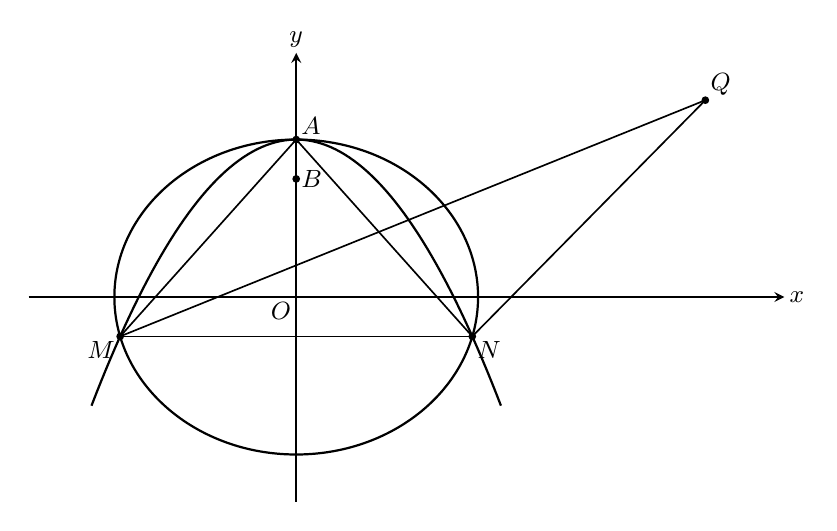
\begin{tikzpicture}[semithick, scale=1.0, every node/.style={inner sep=1.6pt, font=\small}]
  \draw[-stealth] (-3.4,0) -- (6.2,0) node[right] {$x$};
  \draw[-stealth] (0,-2.6) -- (0,3.1) node[above] {$y$};
  % C1 椭圆：a=2.309, b=2
  \draw[thick] (0,0) ellipse (2.3094 and 2);
  % C2 抛物线 x^2 = 4-2y
  \draw[thick,domain=-2.6:2.6,samples=90] plot (\x,{2-(\x)*(\x)/2});
  \fill (0,2) circle (1.4pt) node[above right] {$A$};
  \fill (0,1.5) circle (1.4pt) node[right] {$B$};
  \fill (5.196,2.5) circle (1.4pt) node[above right] {$Q$};
  \fill (-2.236,-0.5) circle (1.4pt) node[below left] {$M$};
  \fill (2.236,-0.5) circle (1.4pt) node[below right] {$N$};
  \draw (-2.236,-0.5) -- (2.236,-0.5);
  \draw (0,2) -- (-2.236,-0.5);
  \draw (0,2) -- (2.236,-0.5);
  \draw (5.196,2.5) -- (-2.236,-0.5);
  \draw (5.196,2.5) -- (2.236,-0.5);
  \node[below left] at (0,0) {$O$};
\end{tikzpicture}
\end{center}
\nopagebreak[4]
\end{question}
\endgroup
\begin{question}
\gkti{22}证明以下命题：

（1）对任一正整数 $a$，都存在正整数 $b,c$（$b<c$），使得 $a^2$，$b^2$，$c^2$ 成等差数列；

（2）存在无穷多个互不相似的三角形 $\triangle_n$，其边长 $a_n$，$b_n$，$c_n$ 为正整数且 $a_n^2$，$b_n^2$，$c_n^2$ 成等差数列。

\end{question}